% Chapter 2

\chapter{Segmentation Neural Networks}

\lhead{Chapter 2. \emph{Segmentation Neural Networks}} % This is for the header on each page - perhaps a shortened title
\label{chp:cbct}
%----------------------------------------------------------------------------------------

\def\:{\hskip0pt} %Definisce un modo veloce per permettere a latex di sillabare correttamente anche parole come 4-connectivity. Il corretto utilizzo è il seguente: 4\:-\:connectivity.

\section{Segmentation using Deep Neural Networks}
\label{sec:segmentation}
Today, deep neural netoworks are the state-of-the-art in many fields, including
image segmentation. In this section, we will briefly review the most common
approaches to segmentation using deep neural networks, and we will discuss the
advantages and disadvantages of each approach.

\subsection{Fully Convolutional Networks}
\label{sec:fcn}
Fully convolutional networks (FCNs) are a class of deep neural networks that
are designed to perform pixel-wise classification. The main idea behind FCNs is
to use a convolutional neural network (CNN) to extract features from the input
image and return an output of the same size as the input image, where each
pixel is assigned a class label. The main advantage of FCNs is that they can be
trained end-to-end, which means that the network can be trained to perform the
classification of each pixel without the need of any post-processing step. On
the other hand, Deep Neural Networks lacks for explainability, which is a major
drawback for medical applications.
The architecture of such networks can be grouped as shown in Figure \ref{fig:fcn_architecture}.
\begin{figure}[ht]
  \centering
  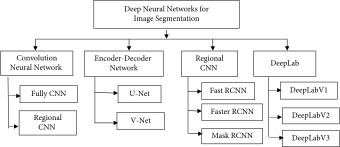
\includegraphics[width=0.8\linewidth]{Images/seg-arch.png}
  \caption{Groups of a segmentation network architecture.}
  \label{fig:fcn_architecture}
\end{figure}

\subsection{Convolutional Neural Networks}
A convolutional neural network or CNN consists of a stack of
three main neural layers: convolutional layer, pooling layer, and fully
connected layer. Each layer has its own role. The convolution layer
detects distinct features like edges or other visual elements in an image.
Convolution layer performs mathematical operation of multiplication of local
neighbours of an image pixel with kernels. CNN uses different kernels for
convolving the given image for generating its feature maps. Pooling layer
reduces the spatial \texttt{(width, height)} dimensions of the input data for the next
layers of neural network. It does not change the depth of the data. This
operation is called as subsampling. This size reduction decreases the
computational requirements for upcoming layers. The fully connected layers
perform high-level reasoning in NN. These layers integrate the various feature
responses from the given input image so as to provide the final results.\\
Different CNN models have been reported in the literature, including AlexNet,
GoogleNet, VGG, Inception, SequeezeNet, and DenseNet. This type of networks were
mostly used for classification, but they have been easily adapted to perform
segmentation.

\subsection{Fully Convolutional Networks}
In fully convolutional network (FCN), only convolutional layers exist. The
different existing in CNN architectures can be modified into FCN by converting
the last fully connected layer of CNN into a fully convolutional layer. This
type of networks can output spatial segmentation map and can have dense
pixel-wise prediction from the input image of full size instead of performing
patch-wise predictions. They can also uses skip connections, when performing upsampling
on feature maps from final layer, these skip connections fuses it with the
feature map of previous layers. The model thus produces a detailed segmentation
in just one go but as drawback they do not have a global context of the image
and the output can be fuzzy close to the boundaries of segmented objects.

\subsection{Encoder-Decoder Networks}
Encoder-decoder based models employ two-stage model to map data points from the
input domain to the output domain. The encoder stage compresses the given input
to a latent space representation, while the decoder predicts the output from
this representation. This latent space representation is a compressed version of
the input image, which is used to generate the output, it have smaller spatial dimension
than the input image but an increased depth. In order to upsample this latent space representation
to the size of the input image, transposed convolutional layers are used.
One of the most popular encoder-decoder networks is the U-Net
\cite{ronneberger2015u}, for which we can find in literature many variants. The
U-Net architecture is shown in Figure \ref{fig:unet_architecture}.
% \begin{figure}[ht]
%   \centering
  % \includegraphics[width=0.8\linewidth]{Images/unet-arch.png}
  % \caption{U-Net architecture.}
  % \label{fig:unet_architecture}
% \end{figure}
U-Net model has a downsampling and upsampling part. The downsampling
section with FCN like architecture extracts features using $3 \times 3$ convolutions to
capture context. The upsampling part performs deconvolution to decrease the
number of computed feature maps. The feature maps generated by downsampling or
contracting part are fed as input to upsampling part so as to avoid any loss of
information. The symmetric upsampling part provides precise localization. The
model generates a segmentation map which categorizes each pixel present in the
image. This type of architecture proposed in 2015 is still widely used today as
it can obtain state-of-the-art resuts.

\subsection{Regional Convolutional Neural Networks}
Regional convolutional network has been utilized for object detection and
segmentation task. The R-CNN architecture presented in [69] generates region
proposal network for bounding boxes using selective search process. These region
proposals are then warped to standard squares and are forwarded to a CNN so as
to generate feature vector map as output. The output dense layer consists of
features extracted from the image and these features are then fed to
classification algorithm so as to classify the objects lying within the region
proposal network. The algorithm also predicts the offset values for increasing
the precision level of the region proposal or bounding box. The processes
performed in R-CNN architecture are shown in Figure 4. The use of basic RCN
model is restricted due to the following:

\subsection{DeepLab}
DeepLab model employs pretrained CNN model ResNet-101/VGG-16 with atrous
convolution to extract the features from an image. The use of atrous
convolutions gives the following benefits:
\begin{itemize}
  \item{It controls the resolution of feature responses in CNNs}
  \item{It converts image classification network into a dense feature extractor
    without the requirement of learning of any more parameters employs
    conditional random field (CRF) to produce fine segmented output}
\end{itemize}
The various variants of DeepLab have been proposed in the literature including
DeepLabv1, DeepLabv2, DeepLabv3, and DeepLabv3+.
In DeepLabv1, the input image is passed through deep CNN layer with one or
two atrous convolution layers. This generates a coarse feature map. The feature
map is then upsampled to the size of original image by using bilinear
interpolation process. The interpolated data is applied to fully connect
conditional random field to obtain the final segmented image.

\section{Dealing with 3D Medical Images}
It is not uncommon in the medical field to deal with 3D images that comes from
CT scans or MRI scans. In this case, a 3D image can be represented as a stack of
2D images and fed them to the network. Each output is then stacked back to
produce the final 3D output. Another approach is to use 3D convolutional
networks. The 3D convolutional network is a generalization of the 2D
convolutional network to 3D data.
In the first case, each 2D layer is indipendend from the others, while in the
second case, the 3D convolutional network is able to learn the spatial
relationships between the different slices of the 3D image.

